\documentclass[twoside]{article}
\usepackage[a4paper]{geometry}
\geometry{verbose,tmargin=2.5cm,bmargin=2cm,lmargin=2cm,rmargin=2cm}
\usepackage{fancyhdr}
\pagestyle{fancy}

% nastavení pisma a češtiny
\usepackage{lmodern}
\usepackage[T1]{fontenc}
\usepackage[utf8]{inputenc}
\usepackage[czech]{babel}

% odkazy
\usepackage{url}

\usepackage{float}
% vícesloupcové tabulky
\usepackage{multirow}
\usepackage{amssymb}
\usepackage{bbold}
\usepackage{amsmath}
\usepackage{mathtools}
\usepackage{commath}

% vnořené popisky obrázků
\usepackage{subcaption}

% automatická konverze EPS 
\usepackage{graphicx} 
\usepackage{epstopdf}
\epstopdfsetup{update}

\graphicspath{{./images}}

% odkazy a záložky
\usepackage[unicode=true, bookmarks=true,bookmarksnumbered=true,
bookmarksopen=false, breaklinks=false,pdfborder={0 0 0},
pdfpagemode=UseNone,backref=false,colorlinks=true] {hyperref}

% Poznámky při překladu
\usepackage{xkeyval}	% Inline todonotes
\usepackage[textsize = footnotesize]{todonotes}
\presetkeys{todonotes}{inline}{}

%https://tex.stackexchange.com/questions/2783/bold-calligraphic-typeface
\DeclareMathAlphabet\mathbfcal{OMS}{cmsy}{b}{n}

% Zacni sekci slovem ukol
\renewcommand{\thesection}{Úkol \arabic{section}}
% enumerate zacina s pismenem
\renewcommand{\theenumi}{\alph{enumi}}

% smaz aktualni page layout
\fancyhf{}
% zahlavi
\usepackage{titling}
\fancyhf[HC]{\thetitle}
\fancyhf[HLE,HRO]{\theauthor}
\fancyhf[HRE,HLO]{\today}
 %zapati
\fancyhf[FLE,FRO]{\thepage}

% údaje o autorovi
\title{Automatické řízení: DÚ 4 - Zpětnovazební smyčky}
\author{Vojtěch Michal}
\date{\today}

\begin{document}

\maketitle

\section{Routhova tabulka}
Nalezněte rozsah zesílení $K_p$, $K_i$ kaskádního kompenzátoru tak, aby uzavřená smyčka s kompenzátorem $K(s)$ a soustavou $G(s)$
s předpisy
\begin{equation}
	\begin{split}
		\label{eq:zadani}
		G(s) &= \frac{1}{(s+2)(s+1)} \\
		K(s) &= \frac{K_p s + K_i}{s}
	\end{split}
\end{equation}
v přímé větvi a jednotkovou zpětnou vazbou byla stabilní. (Použijte Routh-Hurwitzovo kritérium).
\begin{itemize}
	\item Vysvětlete postup výpočtu a uveďte klíčové mezivýsledky.
	\item Nakreslete (v rovině $K_p$, $K_i$) dvourozměrnou oblast hodnot zesílení, pro které je uzavřená smyčka stabilní.
\end{itemize}
\textbf{Řešení:} 
Označme přenos v přímé větvi zpětnovazební smyčky $L(s) = K(s) \cdot G(s)$. Přenosy z rovnice \eqref{eq:zadani} 
vyjádřím standardně jako podíly polynomů v proměnné s. 
\begin{equation}
	\begin{split}
		G(s) &= \frac{b(s)}{a(s)} ~~~~~ \text{, kde} ~ b(s) = 1,~~~~ a(s) = s^2 + 3s + 2 \\
		K(s) &= \frac{q(s)}{p(s)} ~~~~~ \text{, kde} ~ q(s) = K_p s + K_i,~~~~ p(s) = s 
	\end{split}
\end{equation}
Pro přenos $T(s)$ uzavřené zpětnovazební smyčky platí
\begin{equation}
	T(s) = \frac{L(s)}{1 + L(s)} = \frac{\frac{q(s)}{p(s)} \cdot \frac{b(s)}{a(s)}}{1 + \frac{q(s)}{p(s)} \cdot \frac{b(s)}{a(s)}}
	=  \frac{b(s)q(s)}{a(s)p(s) + b(s)q(s)},
\end{equation}
jehož jmenovatel
\begin{equation}
	c(s) = a(s)p(s) + b(s)q(s) = s^3 + 3s^2 + (2+ K_p)s + K_i
	\label{eq:char_polynom}
\end{equation}
je charakteristický polynom uzavřené smyčky.
\subsection{Routh-Hurwitzovo kritérium}
K polynomu třetího stupně přísluší následující Routhovo pole

\begin{centering}
	$\begin{array}{c|cc}
		\centering
		s^3 & a_3 & a_1 \\
		s^2 & a_2 & a_0 \\
		s^1 & R_1  & 0 \\
		s^0 & R_2  &  \\
	\end{array}$, \\ 
\end{centering}

jehož prvky $R_1$ a $R_2$ jsou dány rovnicemi

\begin{equation}
	\begin{split}
		R_1 &= -\frac{1}{a_2} \begin{vmatrix*}
			a_3 & a_1 \\
			a_2 & a_0
		\end{vmatrix*} = \frac{a_1 a_2- a_3 a_0}{a_2} = a_1 -\frac{a_3 a_0}{a_2},\\
		R_2 &= - \frac{1}{R_1} \begin{vmatrix*}
			a_2 & a_0 \\
			R_1 & 0
		\end{vmatrix*} = -\frac{-a_0 R_1}{R_1} = a_0.
	\end{split}
\end{equation}
\newpage
Po dosazení koeficientů charakteristického polynomu z rovnice \eqref{eq:char_polynom} má Routhovo pole tvar 

\begin{centering}
	$\begin{array}{c|cc}
		\centering
		s^3 & 1 & K_p + 2 \\
		s^2 & 3 & K_i \\
		s^1 & -\frac{K_i}{3} + 2 + K_p & 0 \\
		s^0 & K_i &  \\
	\end{array}$. \\
\end{centering}

Routh-Hurwitzovo kritérium je postačující podmínka stability polynomu. Říká, že polynom bude mít tolik nestabilních kořenů, kolik je změn znaménka
v prvním sloupci Routhova pole. Pakliže má být polynom $c(s)$ stabilní, musí mít všechny kořeny v otevřené levé polorovině s a počet změn znaménka v prvním sloupci
Routhova pole tak musí být roven nule. Proto pro zajištění stability uzavřené smyčky musí platit
\begin{equation}
	\begin{split}
		K_i &> 0, \\
		-\frac{K_i}{3} + 2 + K_p > 0 \Rightarrow K_p &> \frac{K_i}{3} - 2.
	\end{split}
\end{equation}
Hodnoty koeficientů $K_p$, $K_i$ řešící tyto nerovnosti (a tedy garantující stabilní zpětnovazební smyčku) jsou vykresleny na obrázku \ref{fig:mozne_hodnoty}.

\begin{figure}
	\centering
	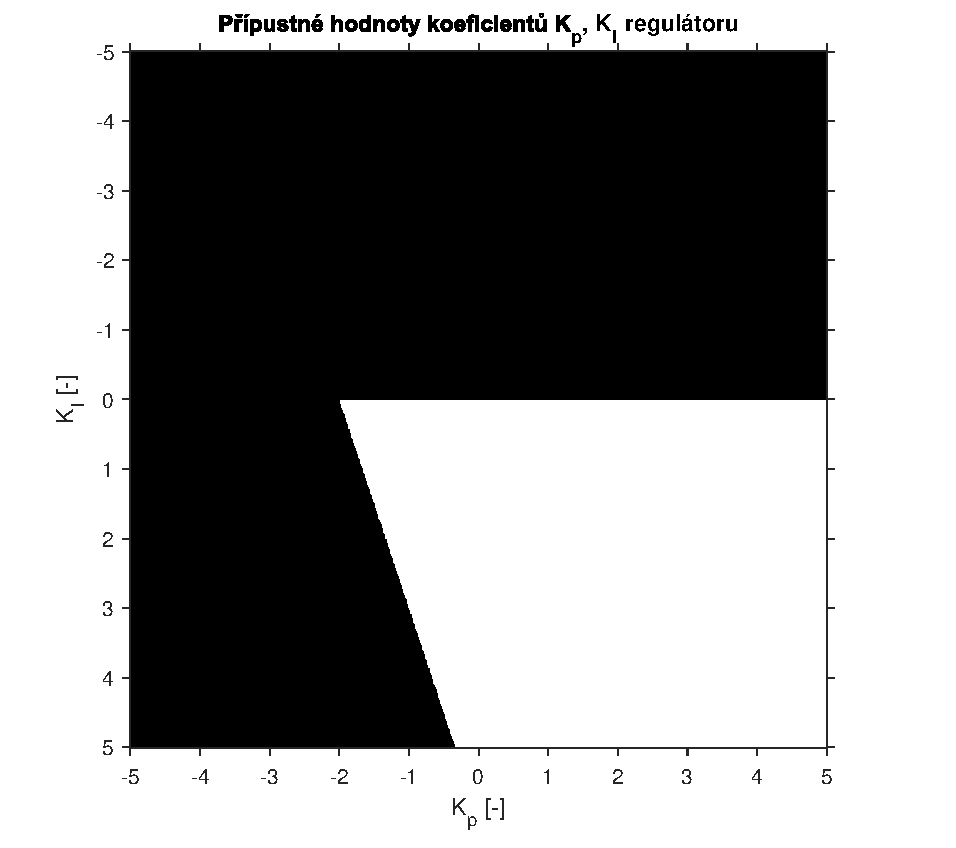
\includegraphics[width=0.8\linewidth]{stabilni_koeficienty.eps}
	\caption{Bíle část roviny $\mathbb{R}^2$ se stabilními koeficienty regulátoru}
	\label{fig:mozne_hodnoty}
\end{figure}

\section{rltool}

Pro datum narození 18. února 2000 mi byla vygenerována přenosová funkce
\begin{equation}
	G(s) = \frac{1}{(s+2)(s+24)}.
\end{equation}
Pro zapojení regulátoru 
\begin{equation}
	K(s) = K_p + \frac{K_i}{s}
\end{equation}
a soustavy $G(s)$ v přímé větvi s jednotkovou zpětnou vazbou
\begin{itemize}
	\item Navrhněte konstanty $K_p > 0$, $K_i > 0$ kompenzátoru pomocí metody root locus s využitím nástroje
	\textbf{rltool} Matlabu tak, aby se póly přenosu uzavřené smyčky nacházely co nejdále vlevo od
	imaginární osy (ten nejbližší byl co nejdál), a přitom jste dodrželi hodnotu poměrného tlumení
	$\zeta = 0.7$.
	\item Vysvětlete váš postup, uveďte hlavní mezivýsledky.
	\item Nakreslete odezvu uzavřené smyčky na jednotkový skok reference.
	\item Jak velká bude odchylka v ustáleném stavu na jednotkový skok reference? 
\end{itemize}

\textbf{Řešení:}

Základní cíle návrhu:
\begin{itemize}
	\item všechny tři póly uzavřené smyčky mají stejnou reálnou část (aby byly všechny co nejdál)
	\item Komplexně sdružené póly leží přesně na přímce příslušné k zadanému poměrnému tlumení $\zeta$
	\item Vše se odehrává v levé polorovině s, aby byla zpětná vazba stabilní
\end{itemize}

V návrhu regulátoru $K(s)$ daného typu pro přenos $G(s)$ máme dva stupně volnosti - polohu nuly a zesílení. Poloha nuly $z_1$ ovlivňuje tvar větví grafu root locus.
Zesílení $K$ ovlivňuje skutečnou polohu pólů uzavřené zpětnovazební smyčky na větvích grafu RL pro danou polohu nuly. Je tedy přirozené nejprve aspoň přibližně umístit nulu.
V nástroji rltool přidáme do kompenzátoru jeden integrátor (jednonásobný pól v $s= 0$) a nulu $z_1$, dále nastavíme \textit{Design requirement} na 
zadané damping ratio $\zeta = 0.7$. Nula musí být jistě reálná, aby všechny polynomy měly reálné koeficienty a root locus tak byl symetrický podle reálné osy.
Máme $n = 3$ pólů, ale jen $m = 1$ nul; $n-m = 2$ větve grafu RL proto směřují do nekončna pod úhlem $\pm 90°$. Pakliže umístím nulu příliš vlevo,
poté bude jen málo ovlivňovat dynamiku systému a větve RL příslušné k pólům v $s = 0$ a $s = -2$ zůstanou blízko imaginární osy.

Pozici nuly tedy volíme tak, aby se průsečík asymptot s reálnou osou
\begin{equation}
	\sigma_a = \frac{\sum p_i - \sum z_1}{n - m} = -13 -\frac{z_1}{2}
\end{equation}
posunul co nejvíce vlevo. To by ideálně vyžadovalo $z_1 > 0$ (ale to je nesmysl, protože nestabilní nula by způsobila, že by se i větve RL dostaly do nestabilní pravé poloroviny s),
vystačíme si s $z_1 > -13$. V této oblasti potom postupným posouváním nuly doprava a sledováním větví root locus lze odhadnout, že optimální pozice bude kolem bodu $-5$.
V této oblasti jsme vlevo od dvou pólů, graf RL bude do nuly vstupovat zleva (jeden pól se s rostoucím zesílením bude přesouvat z -24 směrem k nule),
zatímco dva dominantní póly původně umístěné v bodech 0 a -2 budou v dané oblasti s orstoucím zesílením cestovat více doleva.
Jemným nastavováním konstant získám nastavení regulátoru
\begin{equation}
	K(s) = \frac{255(s+5.2)}{s} = \underbrace{255}_{K_p} + \frac{1}{s} \underbrace{1326}_{K_i},
\end{equation}
pro něž mají všechny tři póly uzavřené smyčky reálnou část rovnu $-8.66$.
Hledané hodnoty konstant proto jsou $K_p = 255$ a $K_i = 1326$. Odezva na jednotkový skok reference je yvkreslena na obrázku \ref{fig:step}.
Díky trojici rychlých pólů dojde za 539 ms k ustálení odezvy na steady state hodnotě 1. Ustálená hodnota regulační odchylky je proto nulová (viz obrázek \ref{fig:step_error}. 
Díky pólu regulátoru vykazuje systém astatistmus prvního řádu a je schopen sledovat jednotkový skok referenčního signálu.

\begin{figure}[htbp]
	\centering
	\begin{subfigure}{0.45\textwidth}
		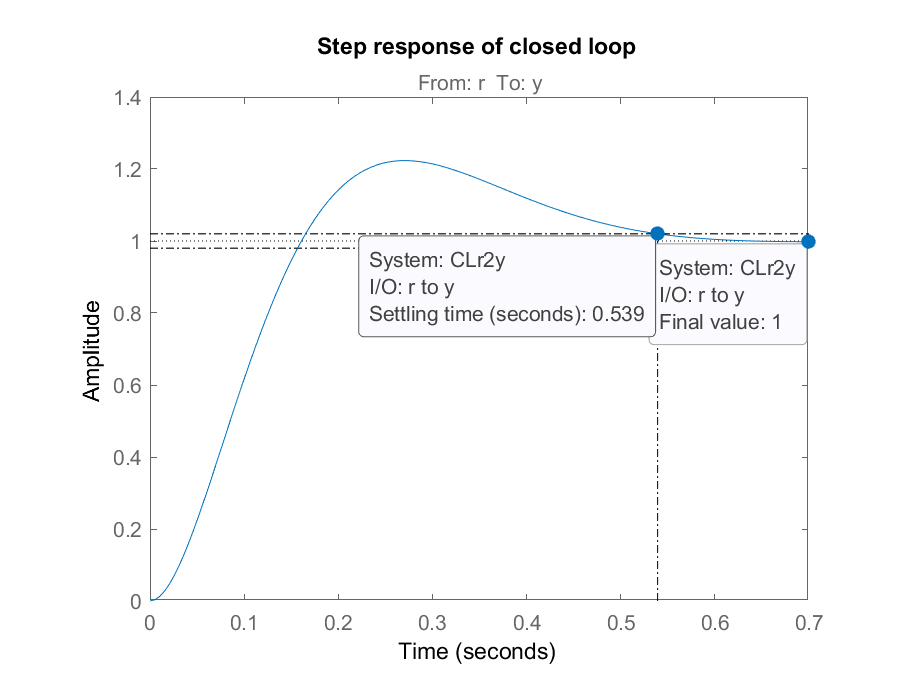
\includegraphics[width=\linewidth]{step_response.eps}
		\caption{Výstup $y(t)$}
		\label{fig:step}
	\end{subfigure}
	\begin{subfigure}{0.45\textwidth}
		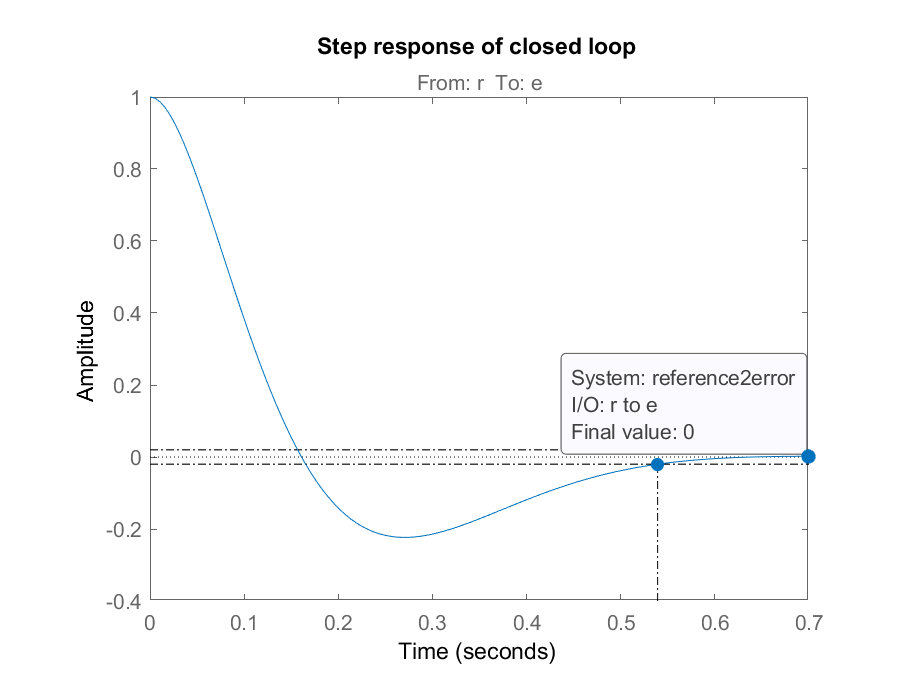
\includegraphics[width=\linewidth]{step_response_error.eps}
		\caption{Regulační odchylka $e(t)$}
		\label{fig:step_error}
	\end{subfigure}
	\caption{Časové odezvy signálů v uzavřené smyčce na jednotkový skok reference $r(t)$}
\end{figure}

\begin{thebibliography}{9}

\bibitem{motivace}
	Robert H. Bishop, Supplementary lectures to book \emph{Modern control systems, 13th edition} \url{https://www.youtube.com/watch?v=CAyWN9ba9J8}

\end{thebibliography}












\end{document}

